% GNUPLOT: LaTeX picture with Postscript
\begingroup
  \makeatletter
  \providecommand\color[2][]{%
    \GenericError{(gnuplot) \space\space\space\@spaces}{%
      Package color not loaded in conjunction with
      terminal option `colourtext'%
    }{See the gnuplot documentation for explanation.%
    }{Either use 'blacktext' in gnuplot or load the package
      color.sty in LaTeX.}%
    \renewcommand\color[2][]{}%
  }%
  \providecommand\includegraphics[2][]{%
    \GenericError{(gnuplot) \space\space\space\@spaces}{%
      Package graphicx or graphics not loaded%
    }{See the gnuplot documentation for explanation.%
    }{The gnuplot epslatex terminal needs graphicx.sty or graphics.sty.}%
    \renewcommand\includegraphics[2][]{}%
  }%
  \providecommand\rotatebox[2]{#2}%
  \@ifundefined{ifGPcolor}{%
    \newif\ifGPcolor
    \GPcolorfalse
  }{}%
  \@ifundefined{ifGPblacktext}{%
    \newif\ifGPblacktext
    \GPblacktexttrue
  }{}%
  % define a \g@addto@macro without @ in the name:
  \let\gplgaddtomacro\g@addto@macro
  % define empty templates for all commands taking text:
  \gdef\gplbacktext{}%
  \gdef\gplfronttext{}%
  \makeatother
  \ifGPblacktext
    % no textcolor at all
    \def\colorrgb#1{}%
    \def\colorgray#1{}%
  \else
    % gray or color?
    \ifGPcolor
      \def\colorrgb#1{\color[rgb]{#1}}%
      \def\colorgray#1{\color[gray]{#1}}%
      \expandafter\def\csname LTw\endcsname{\color{white}}%
      \expandafter\def\csname LTb\endcsname{\color{black}}%
      \expandafter\def\csname LTa\endcsname{\color{black}}%
      \expandafter\def\csname LT0\endcsname{\color[rgb]{1,0,0}}%
      \expandafter\def\csname LT1\endcsname{\color[rgb]{0,1,0}}%
      \expandafter\def\csname LT2\endcsname{\color[rgb]{0,0,1}}%
      \expandafter\def\csname LT3\endcsname{\color[rgb]{1,0,1}}%
      \expandafter\def\csname LT4\endcsname{\color[rgb]{0,1,1}}%
      \expandafter\def\csname LT5\endcsname{\color[rgb]{1,1,0}}%
      \expandafter\def\csname LT6\endcsname{\color[rgb]{0,0,0}}%
      \expandafter\def\csname LT7\endcsname{\color[rgb]{1,0.3,0}}%
      \expandafter\def\csname LT8\endcsname{\color[rgb]{0.5,0.5,0.5}}%
    \else
      % gray
      \def\colorrgb#1{\color{black}}%
      \def\colorgray#1{\color[gray]{#1}}%
      \expandafter\def\csname LTw\endcsname{\color{white}}%
      \expandafter\def\csname LTb\endcsname{\color{black}}%
      \expandafter\def\csname LTa\endcsname{\color{black}}%
      \expandafter\def\csname LT0\endcsname{\color{black}}%
      \expandafter\def\csname LT1\endcsname{\color{black}}%
      \expandafter\def\csname LT2\endcsname{\color{black}}%
      \expandafter\def\csname LT3\endcsname{\color{black}}%
      \expandafter\def\csname LT4\endcsname{\color{black}}%
      \expandafter\def\csname LT5\endcsname{\color{black}}%
      \expandafter\def\csname LT6\endcsname{\color{black}}%
      \expandafter\def\csname LT7\endcsname{\color{black}}%
      \expandafter\def\csname LT8\endcsname{\color{black}}%
    \fi
  \fi
    \setlength{\unitlength}{0.0500bp}%
    \ifx\gptboxheight\undefined%
      \newlength{\gptboxheight}%
      \newlength{\gptboxwidth}%
      \newsavebox{\gptboxtext}%
    \fi%
    \setlength{\fboxrule}{0.5pt}%
    \setlength{\fboxsep}{1pt}%
\begin{picture}(8162.00,5442.00)%
    \gplgaddtomacro\gplbacktext{%
      \csname LTb\endcsname%
      \put(814,704){\makebox(0,0)[r]{\strut{}0}}%
      \put(814,1151){\makebox(0,0)[r]{\strut{}10}}%
      \put(814,1599){\makebox(0,0)[r]{\strut{}20}}%
      \put(814,2046){\makebox(0,0)[r]{\strut{}30}}%
      \put(814,2493){\makebox(0,0)[r]{\strut{}40}}%
      \put(814,2941){\makebox(0,0)[r]{\strut{}50}}%
      \put(814,3388){\makebox(0,0)[r]{\strut{}60}}%
      \put(814,3835){\makebox(0,0)[r]{\strut{}70}}%
      \put(814,4282){\makebox(0,0)[r]{\strut{}80}}%
      \put(814,4730){\makebox(0,0)[r]{\strut{}90}}%
      \put(814,5177){\makebox(0,0)[r]{\strut{}100}}%
      \put(946,484){\makebox(0,0){\strut{}0.00}}%
      \put(1920,484){\makebox(0,0){\strut{}0.10}}%
      \put(2894,484){\makebox(0,0){\strut{}0.20}}%
      \put(3868,484){\makebox(0,0){\strut{}0.30}}%
      \put(4843,484){\makebox(0,0){\strut{}0.40}}%
      \put(5817,484){\makebox(0,0){\strut{}0.50}}%
      \put(6791,484){\makebox(0,0){\strut{}0.60}}%
      \put(7765,484){\makebox(0,0){\strut{}0.70}}%
    }%
    \gplgaddtomacro\gplfronttext{%
      \csname LTb\endcsname%
      \put(176,2940){\rotatebox{-270}{\makebox(0,0){\strut{}$\P\left(\text{power dispatched} \geq \text{reference signal}\right)$, \%}}}%
      \put(4355,154){\makebox(0,0){\strut{}Reference signal for power dispatched to the grid, p.u.}}%
      \csname LTb\endcsname%
      \put(1948,1712){\makebox(0,0)[l]{\strut{}No energy storage}}%
      \csname LTb\endcsname%
      \put(1948,1492){\makebox(0,0)[l]{\strut{}Battery (1), capacity = 0.50 p.u.}}%
      \csname LTb\endcsname%
      \put(1948,1272){\makebox(0,0)[l]{\strut{}Battery (2), capacity = 0.75 p.u.}}%
      \csname LTb\endcsname%
      \put(1948,1052){\makebox(0,0)[l]{\strut{}Battery (3), capacity = 1.00 p.u.}}%
    }%
    \gplbacktext
    \put(0,0){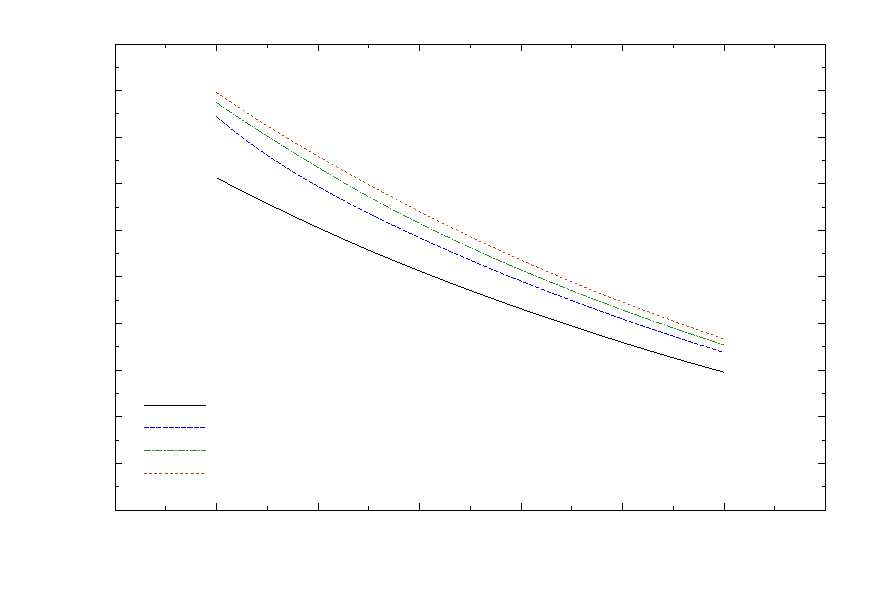
\includegraphics{plot_disp_wind_bess_flat}}%
    \gplfronttext
  \end{picture}%
\endgroup
